\chapter{Airspace, Traffic and Team Flying}\label{cha:airspace}
A database of Special Use Airspace (SUA) can be loaded into XCSoar and
used for both display of the airspace regions as well as detecting
when the glider enters and leaves the regions.

Two airspace files can be set in the configuration settings.  The
first of these is intended for use as the primary SUA database, the
second is intended for use with short-term or changing airspace such
as the airspace defined in NOTAMs.

It is the user's responsibility to ensure that the SUA database
(air\-space file) is up-to-date.

Through a connected FLARM device, the glide computer can also
display information relating to FLARM-equipped nearby traffic
and obstacle threats.

A team code function allows teams of pilots to exchange their
positions via radio in a short code, encoded and decoded by the
computer.

\section{Airspace display}

Local special use airspace regions are drawn on the map as shaded
areas with thick borders.  The colour and pattern of the areas are
specific to different airspace categories and may be configured by the
user.  Depending on the settings, the user may choose to display all
airspaces, only airspaces below a certain altitude, only airspace within a
particular height separation, or only airspace below the glider.
\sketch{figures/airspace.png}

The patterns used to display airspace areas include opaque,
transparent (hollow) and several hatched and stippled patterns.  The
non-opaque patterns are partially transparent with respect to terrain
and topology but are {\em not} transparent with respect to overlapping
airspace.  However, where overlapping airspace occurs, all borders are
visible.  That is, even though airspace patterns are not mutually
transparent, all airspace borders are drawn on top of the airspace
areas.

Both the display and warning of airspace classes can be individually
enabled or disabled by the user as described in
Section~\ref{sec:airsp-filt-dial}.

The default colouring of Class C, D, E and F airspace is consistent
with ICAO charts.

\section{Incursion events}

Three types of events are detected by XCSoar in relation to SUA:
\begin{description}
\item[Predicted incursion] This event is detected when the glider is estimated
to be on a track that will result in entering the airspace at a set
time in the future.  The time is the 'airspace warning time'
configuration setting.

The use of a long term average track in these calculations means that
the system can still predict incursion even when drifting in the wind
when circling.

%{\it DIAGRAM SHOWING DETECTION OF PREDICTED INCUSION WHEN CIRCLING AND
%  CRUISING}

\item[Entering] This event occurs when the glider enters an airspace region.
\item[Leaving] This event occurs when the glider leaves an airspace region.
\end{description}
In all cases, the boundary of the region is defined by maximum and
minimum altitudes or flight levels, as specified in the airspace file.

Airspace warnings are still issued even if the incursion region is
off-screen.

Where a barometric altitude source is available, it is used
preferentially to GPS altitude in detecting airspace incursions.  This
makes the system conform to normal conventions of having airspace
violations based on QNH-adjusted altitude.

\section{Airspace warning levels}

The concept of airspace warning levels is introduced:
\begin{description}
\item[0] Aircraft is outside and distant from airspace.
\item[1] \colorbox{AirspaceYellow}{Aircraft is predicted to penetrate the airspace but is not close.}
\item[2] \colorbox{AirspaceYellow}{Aircraft is predicted to penetrate the airspace and is close to doing so.}
\item[3] \colorbox{AirspaceRed}{Aircraft is inside airspace.}
\end{description}

At all times XCSoar monitors the aircraft relative to all airspace and
maintains warning levels for each.  The airspace warnings are still
filtered according to the airspace filter preferences; such that
certain categories of airspace may be effectively disabled.

The sequence of events when entering an airspace results typically
in three warnings: when near (level 1), when close (level 2), and when
inside (level 3).

\sketch{figures/airspacewarning_2.png}
Whenever the warning level increases (above level 0) for any airspace,
the airspace warning dialog appears, accompanied by a system beep from
Altair or the PDA.  When there are no more airspace regions at warning
levels above 0, the dialog disappears automatically.

\section{Airspace warning dialog}

The airspace warning dialog contains a list of up to 4 individual
warnings.  The list items status background is coloured red if the glider is
inside, and yellow if near.  If the warning is acknowledged, the
text is greyed out.

Each list item occupies two rows, and includes the following details:

\begin{verbatim}
<NAME and Class>               <TOP>   <Inside>
<Time and distance if outside> <BASE>
\end{verbatim} 

The values in the list are continuously updated. 

An example follows:
\begin{verbatim}
Bern TMA Class D                FL100     \colorbox{AirspaceYellow}{near}
35 sec horizontal dist 1300     1750m 
\end{verbatim}

This means that the aircraft is 1300m horizontally separated from the Class D airspace
`Bern TMA', with a base of 1750m and ceiling at FL100.

Another example:
\begin{verbatim}
Bern CTRgld Class C 1350m	    \colorbox{AirspaceRed}{inside}
                    SFC
\end{verbatim}

This means that the aircraft is inside the Class C airspace `Bern
CTRgld', with base of terrain surface and ceiling at 1350m.

At any time, the airspace warning dialog can be opened by selecting
the menu:

\bmenu{Info}\blink\bmenu{Nearest Airspace}

If there were airspace warnings and you are not well outside all airspace, this
menu item redisplays the dialog with the list of airspace warnings.

At any time the airspace warning dialog is show you get the details to an 
airspace by touching on it.

\section{Airspace warning acknowledgement}

When the warning dialog is visible and an airspace warning is active, the
dialog can be closed by pressing ESC.  This has the effect of closing the
warning without actually acknowledging the warning.  

When one or more warnings are visible in the airspace warning dialog,
a warning can be acknowledged by pressing one of the buttons along the bottom
of the dialog.  When the list contains more than one airspace warning,
the rotary button on Altair (or cursor on PDA) can be used to select one
for acknowledgement.

The meanings of the acknowledgement buttons are as follows:
\begin{description}
\item[ACK Warn]  Acknowledge the current warning level.  A new warning will appear
only if the warning level increases.  (Key F5 on Altair)
\item[ACK Space]  Acknowledge all current and future warning levels from this 
particular airspace region while the aircraft is within 2.5km horizontal separation
and 500m vertical separation. (Key F6 on Altair)
\item[ACK Day]  Acknowledge all current and future warning levels from this particular
airspace region for the rest of the flight (specifically, until Altair/XCSoar 
is restarted). (Key F7 on Altair)
\item[Enable]  Cancels an acknowledgement of the airspace, to reactivate all warnings
from this space. (Key F8 on Altair)
\item[Close] Closes the airspace warning dialog, without acknowledging airspace.
  The dialog will re-open automatically if the airspace warning level increases.
\end{description}

Note that not all acknowledgement buttons may be visible for all
warning levels.  In particular, if inside SUA, you do not have the
option to Acknowledge the Warning (ACK Warn), since it is at this
point no longer warning of an impending airspace incursion, but in
fact stating that you are currently inside the airspace.

The general guidelines for using the dialog are:
\begin{itemize}
\item Don't acknowledge a warning if you intend to or must avoid the airspace
\item The warning system beep only occurs when the warning level increases.
\item The warning system is designed to allow circling near an airspace without
  over-stressing the pilot with extraneous warnings.
\end{itemize}

When an airspace region is acknowledged, the region is drawn on the
screen without a pattern.

When the aircraft is predicted to enter an SUA region, or it actually
enters an SUA region, a warning is raised, presented as an audio alert
and a status message describing the type of airspace warning, the SUA
details (including class of airspace, base and ceiling altitude or
flight level, radio frequencies).

%{\it DIAGRAM SHOWING AIRSPACE WARNING}
%\begin{center}
%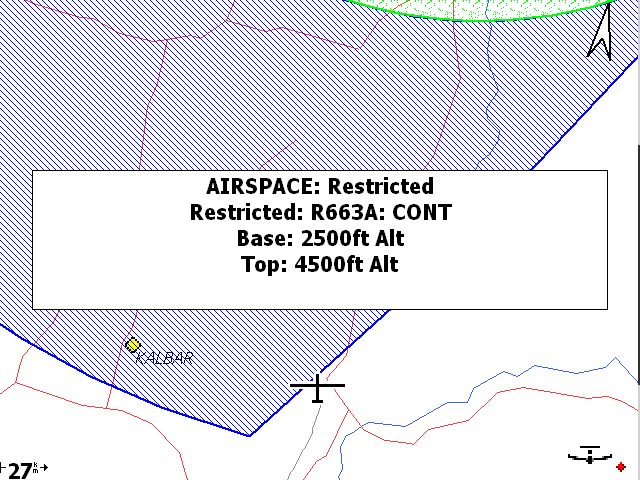
\includegraphics[angle=0,width=\linewidth,keepaspectratio='true']{figures/airspacewarn.png}
%\end{center}

Acknowledged warnings will repeat after a certain time specified as
the 'Acknowledge time' in the configuration settings.

Airspace warning acknowledgements apply to individual SUA regions.
If, for example, a glider enters airspace A and the pilot acknowledges
the warning, and shortly thereafter is predicted to enter airspace B,
an airspace warning for SUA region B will be raised.

\tip If you want acknowledged airspace warnings to not be repeated,
set a very large value for the configuration setting `Acknowledge
time'.

Airspace warnings are automatically cleared when both the current
glider's position as well as the estimated future track are clear
of the airspace.

Simultaneous airspace warnings can occur if the aircraft (or its
estimated future track) penetrates multiple airspace regions.

\section{Airspace queries}

For touchscreen/mouse devices, when an airspace region is visible on
the map area, it may be queried by touching the region on the map.
This brings up a status message containing similar SUA details as is
provided when an actual warning is raised.  Touching the status
message or pressing the enter key makes the message disappear (that
is, it acknowledges the query).  The query returns the details of all
airspace regions when overlapping airspace is visible at the query
location.

Through the button menus, there is another way of querying airspace.
The `Nearest Airspace' query brings up a status message containing SUA
details of the nearest airspace region. 
\begin{quote}
\bmenu{Info}\blink\bmenu{Nearest airspace}
\end{quote}
This returns at most a single airspace region.  The search is limited
to items within half an hour from the aircraft according to flight at
average cross-country speed.

If the glider is outside the airspace, it also describes the distance
and bearing to the nearest point on the airspace perimeter to the
glider.  If the glider is inside the airspace, it also describes the
distance and bearing to the nearest exit.

\section{Airspace filter dialog}\label{sec:airsp-filt-dial}

The Airspace Filter dialog allows warnings and display to be enabled
or disabled for each class of airspace.  

This may be accessed several ways:
\begin{itemize}
\item From the menu \bmenu{Config}\blink\bmenu{Config}\blink\bmenu{Settings
Airspace}
\item From the configuration dialog, menu under
\bmenu{Config}\blink\bmenu{Config}\blink\bmenu{Setup System} then in the
Airspace page, select the button \button{Filter}
\end{itemize}

To use the dialog, move up or down the list and the enter key will
cycle between the various warning and display options.

\begin{center}
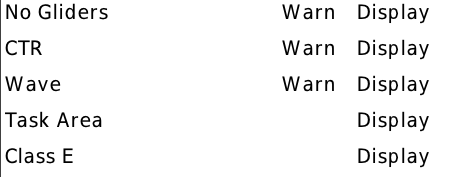
\includegraphics[angle=0,width=0.8\linewidth,keepaspectratio='true']{figures/airspacefilter.png}
\end{center}

Pressing the ``Lookup'' button brings up the airspace select dialog.
This functions similarly to the waypoint lookup dialog, and allows
search based on name, distance, direction, and type (class).  

\begin{center}
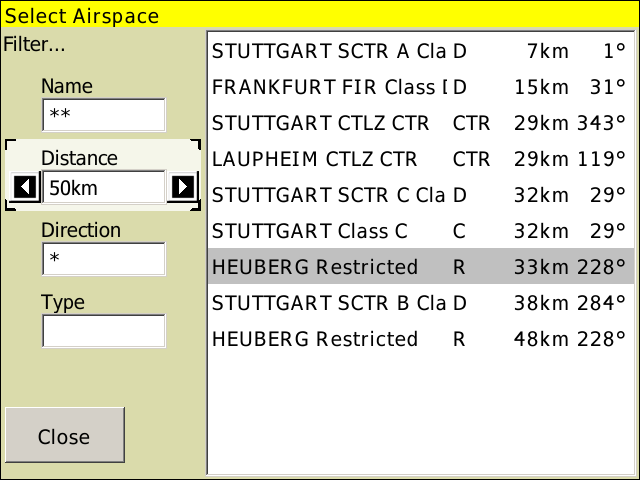
\includegraphics[angle=0,width=0.8\linewidth,keepaspectratio='true']{figures/airspacelookup.png}
\end{center}

Once an airspace item has been located, selecting it will add it to
the airspace management system as acknowledged for the day.  From the
airspace management dialog it is possible to re-enable it again.

\section{Analysis dialog}

The analysis dialog contains a page showing a cross-section of the
airspace.  This is accessed via the menu under
\begin{quote}
\bmenu{Info}\blink\bmenu{Analysis}
\end{quote}

The display shows along the horizontal direction, the
distance from the glider out to 50 km in the direction of the glider's
track; along the vertical direction is height.  The height of the
glider is indicated by a white arrow.  This page is useful to help
visualise complex layering of airspace.

\begin{center}
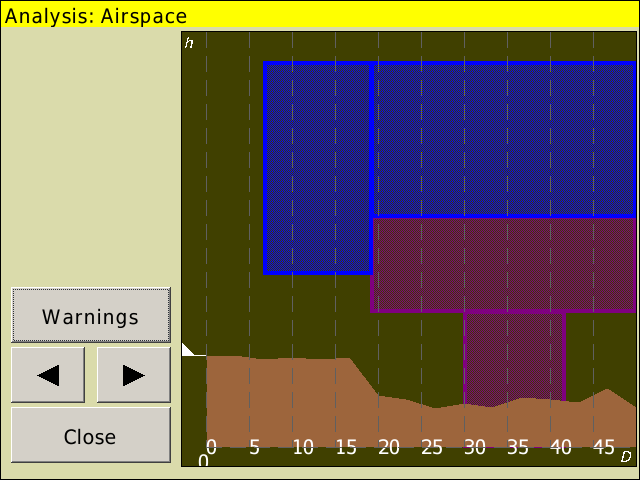
\includegraphics[angle=0,width=0.8\linewidth,keepaspectratio='true']{figures/analysis-airspace.png}
\end{center}

The ``Warnings'' button opens the airspace warning dialog if close to
airspace.

\section{FLARM traffic display}

If connected to a FLARM device, FLARM traffic is displayed on the map
area.  Each FLARM aircraft received is drawn as a dashed red disk.

\warning Do not use XCSoar for collision avoidance, as
FLARM audio devices are much more suitable in assisting the pilot to be
aware of traffic.

Note that unless one is circling, the usual zoom level is such that
FLARM traffic will not be easily distinguished.  When one is circling,
or if the user has North-Up screen orientation, this makes the map display 
a poor aid at helping to locate the traffic.

\subsection*{FLARM map display}

The FLARM targets on the map are drawn as red circles and have coloured 
arrow heads to indicate the direction the FLARM target is
heading, as well as the collision risk \config{flarm-on-map}.  Note that these
arrow heads are oriented according to the display orientation.  For example, if 
the orientation is track-up, then the arrows show the relative track bearing of
the target to the aircraft.  If the orientation is north-up, then the arrows show the
absolute track bearing of the target.

\begin{center}
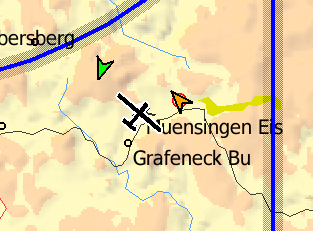
\includegraphics[angle=0,width=0.4\linewidth,keepaspectratio='true']{figures/flarmmap.png}
\end{center}

Display on the map FLARM of aircraft registration or pilot name is
made possible via a look-up of the ICAO aircraft ID of FLARM traffic
in a file.  See Section~\ref{sec:flarm-ident-file} for details on this
file format.  Aircraft with the FLARM privacy flag set will not have
any identification displayed.

\subsection*{FLARM radar}

To remedy this situation, when FLARM traffic is received, the lower
right corner of the screen shows a small radar-style view of the FLARM
traffic from the perspective of the aircraft.  FLARM traffic is
displayed in identical style.

This FLARM display is oriented track-up and a small glider icon
clearly shows that the display is oriented as such.  The scale of the
display is linear up to maximum distance of 2000 meters.  On the
background there are two rings; the first is 1000 meters and the second 
is 2000 meters.  Traffic further away than 2000 meters is drawn at the 2000 meter ring.
\marginpar{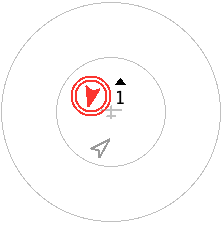
\includegraphics[angle=0,width=\linewidth,keepaspectratio='true']{figures/flarmrose.png}}

All the FLARM displays shows FLARM traffic in colours according to
the threat level, or team and dialog status.  The traffic is coloured:
\begin{itemize}
\definecolor{warning}{rgb}{1,0.64,0}
\definecolor{teammate}{rgb}{0.45,1,0}
\item \textcolor{black} {No color for level 0, no threat.} 
\item \textcolor{warning} { Yellow for level 1, warning.}
\item \textcolor{red} {Red for level 2 and 3, alert.}
\item \textcolor{teammate} {Green for the team mate.}
\item \textcolor{blue} {Blue is the selected target.}
\end{itemize}

For every target above threat level 1 the rough relative hight is shown. The
supplied figure is the absolute hight difference rounded by 100.  A small
triangle indicates that the target is higher or lower than you. The example
radar shows a target approximately 100 meter (for metric altitude) higher.

The FLARM radar-like display, when enabled, can be suppressed when
visible by pressing the enter button (rotary knob on Altair).  If the
FLARM radar is suppressed, pressing the enter button again cancels the
suppression and the radar is shown again.  When new traffic appears in
the radar, or if the FLARM issues a collision warning, the suppression
is cancelled.

When the alert level of the FLARM target indicates a collision
warning, a black line is drawn from the target to the edge of the
radar.  This is done to make it easier to see at a glance which
direction the target is relative to the glider, since when a collision
warning is active, typically the target will be close to the glider.

\subsection*{FLARM Traffic dialog}
Once FLARM has reported traffic and the small radar-style view of the FLARM
traffic gets activated  \config{flarmdisplay} you can tap on the FLARM radar to
enlarge the view to fullscreen size.  This is also accessed via the menu under
\begin{quote}
\bmenu{Info}\blink\bmenu{Info}\blink\bmenu{Info}\blink\bmenu{FLARM Radar}
\end{quote}
The fullscreen FLARM display offers all available information
about the FLARM traffic and depending on the setup it closes by itself, when all
traffic has been gone.

\begin{center}
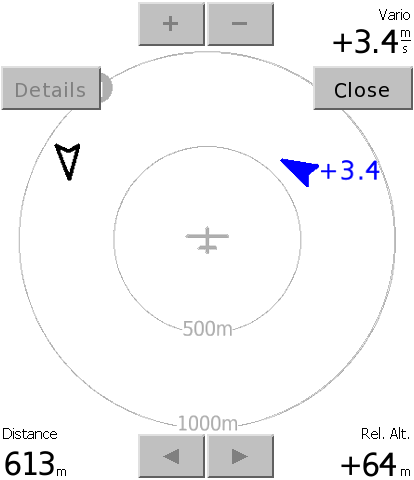
\includegraphics[angle=0,width=0.8\linewidth,keepaspectratio='true']{figures/dialog-flarm1.png}
\end{center}

Only a few controls are on the dialog, from top down:
\begin{description}
\item[North up]  If checked the radar screen is oriented North up, if not the
orientation is Track up.
\item[A. Zoom]  \gesture{Up - Down} Automatic zoom scales the radar screen so
that the targets are perfectly visible. If not checked, the screen must be
zoomed manually. The Up-Down gesture activates the automatic zoom. 
\item[Avg/Alt]  \gesture{Right - Left} The button toggles in-between average
vario and altitude displayed next to the target.
\item[Details]  \gesture{Down - Right} Through the button a separate dialog with
all details to the selected target is accessed. 
\item[+/-]  \gesture{Up/Down} Manually change the zoom from 500 meter to
10000 meter radar range. The zoom gestures also apply here.
\item[$\triangleleft$/$\triangleright$]  \gesture{Left/Right} Select the
previous or next target on the radar, gestures work in the same manner.
\end{description}

\begin{center}
\begin{tabular}{c c}
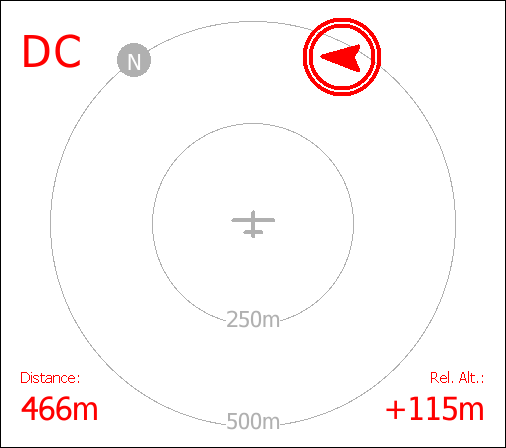
\includegraphics[angle=0,width=0.5\linewidth,keepaspectratio='true']{figures/cut-flarm2.png}&
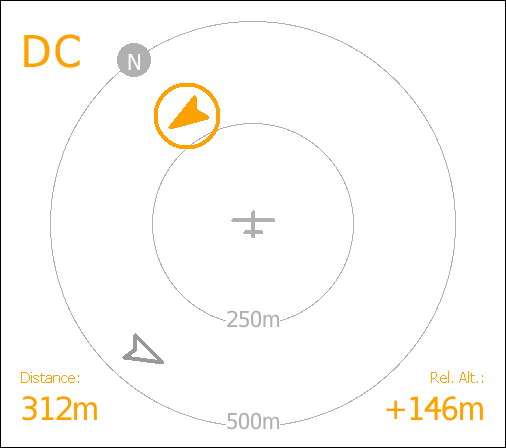
\includegraphics[angle=0,width=0.5\linewidth,keepaspectratio='true']{figures/cut-flarm3.png}\\
\end{tabular}
\end{center}
The three screenshots are taken in a sequence and demonstrate a typical near
pass of e.g. two FLARM equippped gliders. The extra information is colour-coded
in the already mentioned way. In the four corners of the radar screen is
additional info to the selected target displayed:

\begin{description}
\item[Top left]  If available the FLARM Id of the selected target. 
\item[Top right]  Vario of the target, derived from the consecutive altitude
messages.
\item[Bottom left]  The distance to the target.
\item[Bottom right]  The relative hight of the target. 
\end{description}

From the first to the second FLARM snapshot were passed about 15 seconds. The
selected blue target was climbing with 3.4 m/s and had a not as threat
recognised course relation.  Then in the mean time the ``DC'' has turned more to
the left, became an alerting threat and gets now displayed red.  The FLARM
radar switched the zoom from 1000 meter to 500 meter. In snapshot three the
continuously climbing target becomes classified to thread level 1, gets yellow 
coloured and seams to no longer a threat.  


\section{Team flying}

  Team code is a system to allow pilots flying within a team to
  communicate their position to each other in a concise and accurate
  manner.  The principle of the system is that each pilot uses their
  computer to determine a 5 digit code which describes their position
  relative to a common waypoint.  The pilots call each other reporting
  these codes, and entering the codes into the computer allows their
  mates to be located accurately by the computer.

  Support for encrypted team codes will be provided in the future.

  To use team code, all pilots in the team should select a waypoint to
  be used as the reference.  This is done via selecting a waypoint
  from the Waypoint lookup dialog and then pressing the `Set teamcode'
  button in the waypoint details page.

  The teamcode dialog is accessed via the menu:

   \bmenu{Info}\blink\bmenu{Info}\blink\bmenu{Team Code}

  During flight, the pilot can read out his `Own code' from the team
  code dialog to his team mate, in order to report his position.  When
  the pilot hears a code report from a team mate, he presses the \button{Set
  Mate code} button to open the text entry dialog to allow entry of the
  mate's code.

\begin{center}
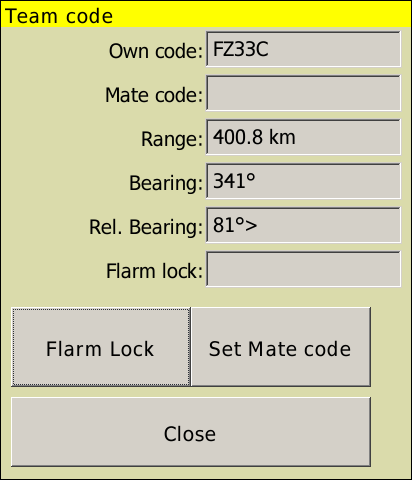
\includegraphics[angle=0,width=0.5\linewidth,keepaspectratio='true']{figures/fig-teamcode1.png}
\end{center}

  After entering the mate's code, the relative distance and
  bearing to the mate is calculated and updated in the dialog.
  
  The \button{Flarm lock} button access the flarm net database. A simple but
  ambiguous lookup for an competition id delivers an flarm id, which alows you
  to ``lock'' your flarm mate from the far.
  



